%\documentclass[11pt,a4paper,fleqn]{scrartcl}

\documentclass[11pt,a4paper,fleqn]{article}
\usepackage{float}  % for [H] placement if needed
\usepackage{amssymb}
\usepackage{graphicx}
\usepackage{amssymb, bm}
\usepackage{svg}
\usepackage{amsmath}
\usepackage{booktabs,dcolumn,caption}
\usepackage{array}
\usepackage{caption}
\usepackage[margin=1in]{geometry}
\usepackage{biblatex} %Imports biblatex package
\usepackage{hyperref}

% Define custom column types for multiline support
\newcolumntype{L}[1]{>{\raggedright\arraybackslash}p{#1}} % left-aligned
\newcolumntype{M}[1]{>{\centering\arraybackslash}m{#1}}   % centered
\newcolumntype{R}[1]{>{\raggedleft\arraybackslash}p{#1}}  % right-aligned

\captionsetup{labelsep=newline, singlelinecheck=false, skip=0.333\baselineskip}

\begin{document}

\title{Are gut microbial communities process based modeled?}

\author{
	\small{%
		\href{https://orcid.org/}{Sabrina Spigno}\(^{1, *}\),
		\href{https://orcid.org/}{}\(^1\)
		\href{}{}\(^{1, *}\)
	}
}
\date{2024/2025}

\maketitle  

\section{Introduction}
\begin{figure}[ht]
	    \centering
    \includegraphics[width=0.8\textwidth]{"FIGS/Slide1.png"} % Replace with your image filename
    \caption{\label{fig:sample} The number of article found in Scopus in the 3 queries (see attached table S1) with different thematic areas.}
    
\end{figure}


Over the past decade, interest in the gut microbiota has increased significantly, 
particularly regarding its role in human health \cite{adler_life-cycle_2007}.
This growing attention has extended to the development of mathematical models 
aimed at understanding the complex dynamics of gut microbial communities. 
Among these models, process-based models (PBMs)—those grounded in mechanistic biological 
assumptions—remain comparatively underrepresented.

To assess the current landscape of mathematical modeling in this field, 
I conducted a systematic literature search using the terms gut microbiota, health 
and mathematical modeling. After filtering out review articles, 
the remaining studies were categorized based on their modeling approach. 
A substantial number involved in vitro or in vivo experimental systems, 
which, while valuable, do not fall under the definition of mechanistic 
process-based models. 
A considerable proportion of studies employed genome-scale metabolic models (GSMMs), 
which typically follow a top-down approach. These models are constructed from annotated genome 
sequences and aim to represent all known metabolic reactions encoded in an organism’s genome.
GSMMs are structured as large stoichiometric matrices where rows correspond to metabolites and columns to biochemical reactions. 
The core assumption is that, under steady-state conditions, 
the net production or consumption of each internal metabolite is zero. 
Using this structure, one can apply flux balance analysis (FBA) to compute 
feasible metabolic flux distributions that optimize a given objective function (e.g., biomass production or energy yield), 
subject to stoichiometric and thermodynamic constraints.
However, PBMs—those aimed at capturing dynamic biological processes over time—comprised the smallest category.
Unsurprisingly, most ODE-based models used in gut microbiota research were the generalized Lotka–Volterra (gLV) model.
The gLV framework models species interactions as direct, additive, and pairwise—meaning that the impact of one species
 on another is assumed to be independent of other species in the system, and the total effect is simply the sum of all pairwise contributions.

Within the PBMs identified, the majority utilized ordinary differential equations (ODEs) (n = 40), while fewer employed partial differential equations (PDEs) (n = 5) or individual-based models (IBMs) (n = 6).
\indent To better understand the state of the field,
I conducted a systematic literature search using
the query terms gut microbiota and mathematical modeling.
After filtering out review articles, I classified the remaining studies
by the modeling approach used.
The majority were in vitro or in vivo experimental studies, that are not correctly process based models.
An also big number were represented by genome-scale metabolic model (GSMMs), that uses the 
top-bottom approach were the smallest represented.
Of the PBMs, the dominant frameworks were based on ordinary differential equations (ODEs) (n = 40), with fewer using partial differential equations (PDEs) (n = 5) or individual-based models (IBMs) (n = 6).

\indent Unsurprisingly, most ODE-based models used in gut microbiota research
are variants of the generalized Lotka–Volterra (gLV) model [add citations here, e.g., Emil's paper and others].
The gLV formalism assumes that species interact via direct, additive, pairwise interactions.
That is, the effect of one species on another is independent of the presence or state of other species,
and the total effect is simply the sum of these pairwise influences.
\indent However, recent critiques have highlighted several limitations of pairwise gLV models:
\begin{itemize}
	\item These models lack memory, mediation effects, or conditional dependencies, and typically converge to a single equilibrium point, that is for community population, usually, unstable.
	\item Immigration is often artificially required in simulations involving large communities to prevent extinctions and maintain coexistence. This raises questions about the ecological realism of the model.
	\item The assumption of a single fixed equilibrium can be too simplistic given the observed multistability in gut microbiota compositions.
	\item Pairwise gLV models fail to account for higher-order interactions and environmental mediators, such as metabolites that are produced or consumed by multiple species. These oversights limit the models' ability to capture emergent community-level phenomena.
	\item Extensions such as the delayed gLV [add citation] have been proposed to address some of these issues, incorporating time delays that can arise from metabolite production or signaling pathways.
	\item I can also talk about the data that are used to calibrate this model, and also that for example usaually just few species are described and most of the species are grouped as Others. when talking about large community models it make sense, because the numbers are very high and in most of the cases there are not enough collection in time.
	

\end{itemize}

\begin{figure}[h]
	    \centering
    \includegraphics[width=0.8\textwidth]{"FIGS/Slide5.png"} % Replace with your image filename
    \caption{\label{fig:sample1} The number of articles divided by several methods included in the words used to find the Query 3. Others represents computational framework that were not categorized into genome scaled metabolomics model, in vitro cultured models, in vivo models, process-based model and statistics models. In particular into those classification there are power laws model, coarse grained models, specific network information gain.}
    
\end{figure}


Given these limitations, there is a clear need for more comprehensive and mechanistic alternatives to pairwise gLV models. 
One promising avenue is the inclusion of autotoxicity, where a species alters its environment in a way that negatively impacts its own growth. This introduces additional state variables and feedback mechanisms that allow the model to capture more realistic community dynamics.

We hypothesize that incorporating autotoxicity into PBMs may offer several advantages:

\begin{enumerate}
\item it has a biological meaning observed in nature (cit. )
\item It enables stable coexistence of species, even under strong interspecies competition.
\item It supports the emergence of multiple equilibria, allowing for both diverse and collapsed community states.
\item It may better reflect ecological patterns observed in the gut microbiota, such as dominance by a single species (e.g., during dysbiosis or diarrhea) or stable coexistence in the absence of constant immigration.
\end{enumerate}
\begin{figure}[h]
	    \centering
    \includegraphics[width=0.8\textwidth]{"FIGS/Slide6.png"} % Replace with your image filename
    \caption{ \label{fig:sample2} The number of articles divided by several methods included in the words used to find the Query 3. Others represents computational framework that were not categorized into genome scaled metabolomics model, in vitro cultured models, in vivo models, process-based model and statistics models. In particular into those classification there are power laws model, coarse grained models, specific network information gain.}
   
\end{figure}


\begin{figure}[h]
	    \centering
    \includegraphics[width=0.8\textwidth]{"FIGS/Slide7.png"} % Replace with your image filename
    \caption{\label{fig:sample3} The number of articles divided by several methods included in the words used to find the Query 3. Others represents computational framework that were not categorized into genome scaled metabolomics model, in vitro cultured models, in vivo models, process-based model and statistics models. In particular into those classification there are power laws model, coarse grained models, specific network information gain.}
    
\end{figure}

What will be done in this chapter:
\begin{itemize}
	\item Draw a model that account for two variables, the species and the autotoxicity
	\item explore this model dynamic for single species, two species and community
\end{itemize}



\captionsetup{labelsep=newline,
              singlelinecheck=false,
              skip=0.333\baselineskip}
\newcolumntype{d}[1]{D{.}{.}{#1}} % "decimal" column type
\renewcommand{\ast}{{}^{\textstyle *}} % for raised "asterisks"




\begin{table}[h]
\caption{Comparison of modeling approaches applied to gut microbiota.}
\label{tab:modeling_approaches}
\small
\begin{tabular}{@{\extracolsep{2pt}} L{2cm} L{2cm} L{3 cm} L{4cm} L{4 cm}}
\toprule
\textbf{Methods} & \textbf{Symbol} & \textbf{Description} & \textbf{Strengths/Weaknesses} & \textbf{Application in gut microbiota} \\
\midrule
Differential equation based models 
& ODE or PDE 
& Mathematical model simulating variables change in time 
& Strengths: can make both predictions pertaining to dynamics and long-term equilibrium states. Weakness: requires parameters that are unknown or difficult to measure.
& To model monocultures or simple co-culture systems consisting of a few gut microbial species. To model microbial community estimating the growth rates of species and interaction strength. \\
\addlinespace
Individual based models 
& IBM 
& The study of a single microbial species behaviour to describe the whole system 
& Strengths: model heterogeneous populations, flexibility in mechanistic resolution. Weakness: not good for homogeneous data, can be computationally expensive, hard to scale and difficult to fit to a system.
& Simulate gut microbial key species behaviour \\
\addlinespace
Genome-scale metabolic models 
& GSMMs 
& Mathematical structures describing all reactions associated with metabolic genes in the organism’s genome.
& Strength: useful for understanding essential genes, inter-species interaction, and culture media. Weakness: requires high-quality genomic data and doesn’t capture dynamics meaningfully.
& Study of species-specific metabolisms and metabolic interactions within gut microbial communities. \\
\bottomrule
\end{tabular}
\end{table}

\begin{table}[ht]
\caption{Summary of modeling approaches applied to gut microbiota (minimal version).}
\resizebox{\textwidth}{!}{%
\begin{tabular}{L{2.2cm} L{3cm} L{4cm} L{4.2cm} L{3cm} L{3cm}}
\toprule
\textbf{Model} & \textbf{Model dynamics} & \textbf{Microbial taxa} & \textbf{Organisms} & \textbf{Substrate} & \textbf{Refs} \\
\midrule

ODE & gLV & / & / & implicit & 10.1016/j.ecolmodel.2021.109733 \\
& gLV & OTUs & Bacteroides, Firmicutes, Proteobacteria, Verrucomicrobia & implicit & 10.1073/pnas.1311322111 \\
& cLV & genera &und. Enterobacteriaceae, Blautia, Barnesiella, und. Uncl. Mollicutes, und. Lachnospiraceae, Akkermansia, Clostridium difficile, uncl. Lachnospiraceae, Coprobacillus, Enterococcus, Others
& implicit & \cite{martin_vitro_2018} 10.1103/PhysRevE.99.032403 \\

\addlinespace

 & Monod kinetics & species & Bacteroides thetaiotaomicron, Methanobrevibacter smithii, Eubacterium rectale 
 & acetate, carbon dioxide, polysaccharides
& 10.1038/s41598-023-48524-4 \\
 & Contois + Monod kinetics & species & 
Generalist biomass in lumen and in mucus (Bacteroides thetaiotaomicron), Mucin specialist biomass in lumen and in mucus (Akkermansia muciniphila)
&  Dietary fiber in lumen, Mucin in lumen, Dietary fiber dirived sugar in lumen, Mucin derived sugar in lumen, Mucin glycoprotein in mucus, Dietary fiber-derived sugar in mucus, Mucin-derived sugar in mucus
& 10.1016/j.jtbi.2024.111824 \\

\addlinespace

& Monod growth rate & species and family & Bacteroides spp., Ruminococcus bromii, Ruminococcus albus, Ruminococcus flaviescens, Bifidobacterium spp., Collinsella aerofaciens, Eubacterium rectale, Roseburia spp., Faecalibacterium prausnitzii, Veillonella spp., Megasphera elsdenii , Eubacterium hallii, Anaerospires spp., Blautia hydrogenotrophica, Methanobrevibacter smithii
 & Acetate, propionate, succinate, non-butyrate forming starch, non butyrate forming fiber, lactate, methane 
 & 10.1111/1462-2920.12599 \\
& Monod growth rate & species & Eubacterium hallii, Anaerostipes coli& / & 10.1111/j.1574-6941.2011.01085.x \\

\addlinespace
PDE & / & / &  hydrogen polysaccharides degraders bacteria, lactate degraders bacteria, acetogenesis pathway bacteria, methanogenesis pathway bacteria & liquid, digestive residue, mucus, polysaccharides, monosaccharides, lactate, acetate, propionate, butyrate, methane, carbon dioxide 
 & 10.1016/j.jtbi.2018.12.009 \\

\addlinespace
IBM & — & genera & Bacteroides, Clostridium, Bifidobacterium, Desulfovibrio & Inuline, Glucose, Lactose, Fructooligosaccharides, Chondroitin sulphate, Lactate
 & (\cite{lin2018gutlogo} Lin et al., 2018, DOI: 10.1371/journal.pone.0207072; DOI: 10.1016/j.mehy.2015.01.027) \\
& — & — & Bacteria type 1 and 2 (consumer chain) & Polysaccharides, Propionate, Acetate, Butyrate & (Shashkova et al., 2016, DOI: https://doi.org/10.1371/journal.pone.0148386) \\

\bottomrule
\end{tabular}
}
\end{table}




\clearpage
\section{Model 1 description}
\subsection{Equations}
The model version 1 with explicit dynamics for species-specific autotoxicity reads:
\begin{equation}
\frac{dn_i}{dt} = n_i \left(r - \rho a_i - \sum_{j \neq i} C_{j} n_j + \lambda \right), \label{eq:1}
\end{equation}

\begin{equation}
\frac{da_i}{dt} = \beta n_i - \delta a_i, \label{eq:2}
\end{equation}

The same equations but in log-scale:

\begin{equation}
\frac{dlog(n_i)}{dt} =  \left(r - \rho a_i - \sum_{j \neq i} C_{j} n_j + \frac{\lambda}{n_i} \right), \label{eq:3}
\end{equation}

\begin{equation}
\frac{dlog(a_i)}{dt} = \beta\frac{n_i}{a_i} - \delta , \label{eq:4}
\end{equation}
\subsubsection{Parameters}
In this model, there are two state variables for each species \( i \):
\begin{itemize}
    \item The variable \( n_i \) represents the population abundance of species \( i \).
    \item The variable \( a_i \) represents the concentration of an autotoxin produced by species \( i \).
\end{itemize}

The dynamics of the system are governed by species growth and the effect of autotoxicity. The key parameters of the model are:
\begin{itemize}
    \item \( r \): intrinsic growth rate of the species,
    \item \( \rho \): sensitivity of the species to its own autotoxicity,
    \item \( \beta \): production rate of autotoxicity,
    \item \( \delta \): dilution rate of autotoxicity.
    \item \( \lambda \): immigration rate.
\end{itemize}

The inter-species interactions are captured by the term
\[
\sum_{j = i} C_{j} n_j,
\]
where \( C_j \) represents the effect of species \( j \) on species \( i \). 
The interaction coefficients \( C_j \) are assumed to be drawn from a 
normal distribution with mean \( \mu \) and standard deviation \( \sigma \), 
that is:
\[
C_j \sim \mathcal{N}(\mu, \sigma^2). 
\]
with $C_{ii} = 1$ for all $i$. An alternative setting is where $C_{ii} = 0$, attributing diagonal contributions solely to autotoxicity.

The corresponding GLV model for comparison is:

\begin{equation}
\frac{dn_i}{dt} = n_i \left(1 - \rho \frac{\beta}{\delta} n_i - \sum_j C_{ij} n_j \right), \label{eq:5}
\end{equation}

using the same $C_{ij}$ statistics, optionally setting $C_{ii} = 0$.

\subsection{Equilibrium points and stability}
In the limit of fast autotoxin dynamics relative to population dynamics, both models converge.
The equilibrium values $n_i^*$ are the same in both models..

Solving Eq. \eqref{eq:2} at stationarity:
\begin{equation}
a_i^* = \frac{\beta}{\delta} n_i^*, \label{eq:6}
\end{equation}

which gives:

\begin{equation}
n_i^* = \frac{1 - \sum_{j \ne i} C_{ij} n_j^*}{1 + \rho \beta / \delta}, 
\label{eq:7}
\end{equation}

To check feasibility, solve:

\begin{equation}
\sum_j \tilde{C}_{ij} n_j^* = 1, 
\label{eq:8}
\end{equation}

with $\tilde{C}_{ij} = C_{ij}$ for $j \ne i$ and $\tilde{C}_{ii} = C_{ii} + \rho \beta / \delta$.

\subsubsection{Jacobian Analysis}

Let $J$ be the Jacobian at equilibrium. For the GLV model:

\begin{equation}
J_{ij} = -C_{ij} n_i^*, \quad j \ne i,
\end{equation}
\begin{equation}
J_{ii} = -(1 + \rho \beta / \delta) n_i^*.
\end{equation}

For the model with explicit autotoxicity:

\[
J = 
\begin{bmatrix}
J_{nn} & J_{na} \\
J_{an} & J_{aa}
\end{bmatrix},
\]

with components:

\begin{align}
J_{nn, ij} &= -C_{ij} n_i^*, \quad i \ne j, \\
J_{nn, ii} &= -n_i^*, \\
J_{na, ij} &= 0, \\
J_{na, ii} &= -\rho n_i^*, \\
J_{an, ij} &= 0, \\
J_{an, ii} &= \beta, \\
J_{aa, ij} &= 0, \\
J_{aa, ii} &= -\delta.
\end{align}

The GLV Jacobian depends only on the combination:

\begin{equation}
\frac{\rho \beta}{\delta},
\end{equation}

while in the explicit model, $\rho$, $\beta$, and $\delta$ appear separately, potentially yielding distinct stability properties.
The stability properties can be
different.
\clearpage

\begin{figure}[h]
    \centering
    \includegraphics[width=0.8\textwidth]{"EigenvaluesglvAutotox1.png"} 
    \caption{\label{fig:EigenvaluesglvAutotox1} Spectrum of the eigenvalues for the Jacobian matrix of the GLV model with explicit
dynamics for the autotoxin (blue) and the one for the equivalent GLV (orange). Parameters are,
number of species S = 100, $\mu$ = 0.01, $hat{\sigma}$ = 0.05, $\rho$ = $\delta$/$\beta$. Large negative outliers are not represented
in the plots.}
\end{figure}

 In Figure \ref{fig:EigenvaluesglvAutotox1} we show the spectrum of the eigenvalues of the Jacobians of the two model
compared. If $\rho$ = $\delta$/$\beta$, in such a way that the GLV model has always the same behaviour, we see
that changing $\beta$ does not change the stability properties of the system while changing $\delta$ has a
string effect. For low values (to be quantified) of  $\delta$, the model has worst stability properties with
respect to GLV, with the largest eigenvalue closer to 0. For relatively higher values the model
become, better, regarding stability properties Finally, for large values of $\delta$, i.e. fast autotoxin
dynamics, the system tend to coincide.
Here we focused on feasible and stable parts of the parameter space in order to avoid solving
explicitly the dynamics to find the equilibrium values, but the consideration should be extendable
closer to the instability threshold.


\clearpage

\subsection{Simulations- species dynamics in time}

All numerical simulations were carried out in python (Python 3.12.3) using the numpy and scipy packages. 
To simulate both the version of the autotoxicity model, a try except block was used to first try two standard adaptive ODE solver of scipy, RK45 and LSODA 
and then a fixed time integrator with small time step $\Delta$t=0.05. 
All the simulations were computed using the logarithm of the abundances to guarantee the positivity of all abundances at all times.
We assume that the interaction matrix is 0, the intrinsic growth rate r is 1 for all the species and that the increasing rate of autotoxicity $\beta$ is also 1 and equal for all the species.
In the simulations, we change the parameter $\delta$, $\rho$, $\mu$ and $\sigma$.
\subsubsection{single species}
\begin{figure}[h]
    \centering
    \includegraphics[width=0.8\textwidth]{"Model01species.png"} % Replace with your image filename
    \caption{\label{Model01species} Simulation of single species in the first version of the model of explicit dynamics of autotoxicity.
    Species (Solid line) and Autotoxicity (Dashed line) dynamics in log space with $\delta$=0.01 on the left and $\delta$=5 on the right.}
\end{figure}

\begin{figure}[h]
    \centering
    \includegraphics[width=0.8\textwidth]{"model1_1speciesRHO.png"} % Replace with your image filename
    \caption{\label{model1_1speciesRHO} Simulation of single species in the first version of the model of explicit dynamics of autotoxicity.
    Species (Solid line) and Autotoxicity (Dashed line) dynamics in log space with $\rho$=0.01 on the left and $\rho$=2.5 on the right.}
    
\end{figure}

In Figure \ref{Model01species} the simulation of single-species model is showed in two cases, with low diluition rate $\delta$= 0.01 and with high diluition rate $\delta$=5. 
 High values of $\delta$ corresponds to low levels of autotoxicity, representing fast autotoxin dynamics. 
 In this conditions, the system reaches the equilibrium rapidly and without oscillations.
Those results support the findings present in Figure \ref{fig:EigenvaluesglvAutotox1} where we showed that
increasing $\delta$ leads to convergence of the autotoxicity and the gLV model.
Additionally, the single-species model were simulated also varying the sensititvity of the species to autotoxicity $\rho$ from 0.01 to 2.5 (Figure \ref{model1_1speciesRHO})
For high values of  $\rho$, the system reaches its fixed point with damped oscillations, with a similar behaviour
observed when decreasing $\delta$. For lower values of $\rho$ the system reaches
the fixed point with slower oscillations. Those results highlight the analogous dynamical
roles of $\rho$ and $\delta$ in controlling the system's stability.

\subsubsection{two species}
In the two species dynamics we simulated different scenarios by changing the parameter $\rho$ and the interaction matrix between the two species. 
In detail, the simulations resulted from values of $\rho$=[0.1, 0.8, 1],  ${C}_{12}$= [-0.3, 0.2, 0.2] and ${C}_{21}$=[-0.2, 1.2, 0.3],
while the other parameters, $\delta$=0.01 and $\lambda$=1e-8 were fixed and the initial conditions were the same for both the species [0.05, 0.05] and the autotoxicities [0.0, 0.0].
\begin{figure}[h]
    \centering
    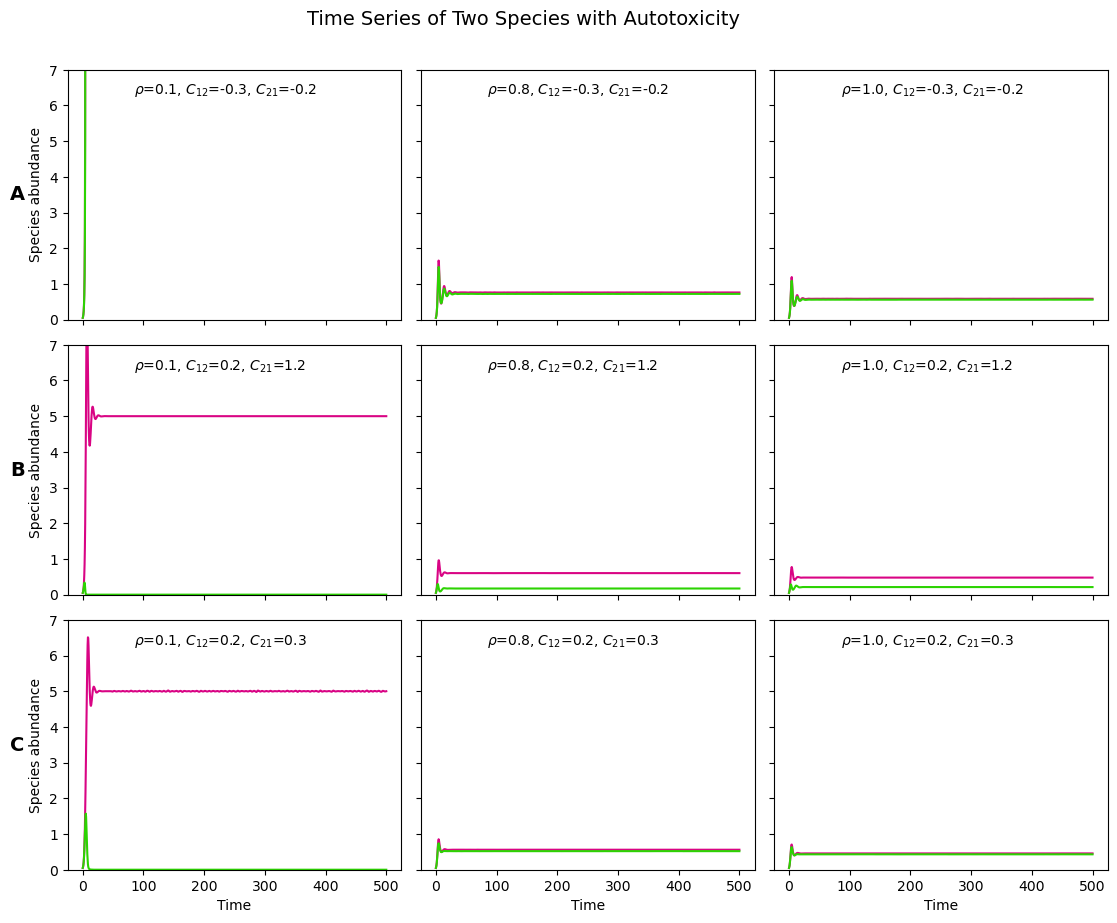
\includegraphics[width=\linewidth]{twospeciesModel1.png}
    \caption{\label{simulationTwoSpeciesModel0} Simulation of two species dynamics model. Species 1 (green) and Species 2 (Pink) dynamics in linear space.}
\end{figure}

We observe that in the first column of Figure \ref{simulationTwoSpeciesModel0}, 
corresponding to low sensitivity to autotoxicity, 
the system fails to reach a stable solution when both species exhibit mutual cooperation (panel A).
This instability arises due to the fact that the species does not have any limitation, leading the system to explode.
In contrast, under competitive interaction (Figure \ref{simulationTwoSpeciesModel0}, B and C) 
the model does reach steady state. However, in these cases, the more competitive species
dominates, driving the other species to extinction. 
As the sensitivity to the autotoxicity increases, (Figure \ref{simulationTwoSpeciesModel0}, column 2 and 3), 
the system exhibits qualitatively different behaviour, where extinction is prevented across all the interaction types
and both species are able to cohexist.
\clearpage

\section{Autotoxicity vs gLV- how to make a proper parallelism: 2nd version of the model}
Establishing a direct parallel between the autotoxicity-based model and the Generalized Lotka Volterra (gLV) framework is not straightforward, 
primarily because the former involves two state variables per species, while the latter relies on a single-variable formulation. 
In the limit of fast autotoxicity dynamics, corresponding to large values of the dilution rate $\delta$, 
the behavior of the autotoxicity model tends to converge to that of a gLV system.

However, in the current formulation, $\rho$ and $\beta$ also nfluence the system's equilibrium, making it
not trovial to isolate the effect of autotoxicity by simply 
adjusting $\delta$. 

Moreover, the presence of multiple parameters introduces complexity and is probably
unuseful. Notably, the single-Species simulations suggest that the sensitivity to the autotoxicity $\rho$ and the 
diluition rate $\delta$ play analogous roles in determining the system's stability. 
In fact, both the parameters modulate the damping oscillations and the convergence to equilibrium. 
The easiest way to compare the two systems, would be to have a comparative framwork,
where we exactly know what is the dynamic. For example, one could begin with the gLV model and 
examine how its behavior changes upon introducing an additional state variable representing autotoxicity. 

Our starting point is the GLV:
\begin{equation}
\dot{n}_i = n_i\left( r_i - C_{ii} n_i - \sum_{j(\neq i)} C_{ij} n_j \right)
\label{eq:glv1}
\end{equation}
This is a phenomenological and not a mechanistic model. 
The intra-specific suppression term, for instance, is meant to roughly capture the net effect of a variety of processes: conspecifics competition over resources, space, the effect of pathogens -- and autotoxicity. 

We should therefore think of the autotoxicity model as unpacking some of the biological processes hidden in the phenomenological self-suppression term, 
rather than adding new mechanisms on top of what's already represented by the GLV. This gives the generalization:
\begin{equation}
\dot{n}_i = n_i\left( r - C_{ii} h(n_i,a_i) - \sum_{j(\neq i)} C_{ij} n_j \right),
\end{equation}
with $a_i$ the autotoxin concentration. 
We want to preserve, in a sense, the interpretation of $C_{ii}$ as the net strength of self-suppression effects. 
The function $h(n,a)$ should partition these effects into a fraction $\gamma$ due to autotoxicity and the remaining fraction $1-\gamma$ due to the other implicit causes.

If we assume that individuals die due to autotoxicity at a rate proportional to the autotoxin concentration, then $h(n,a)$ is linear in both arguments. To have a notion of partitioning between $a$ and $n$, we must find what amount of $n$ constitutes an "equivalent" amount of $a$.

To this end, consider the autotoxicity dynamics. Production occurs at a per capita rate $\beta$ and degradation/dilution at a rate $\delta$:
\begin{equation}
\dot{a}_i = \beta n_i - \delta a_i.
\end{equation}
The formal solution is:
\begin{equation}
a_i(t) = \frac{\beta}{\delta} \int_{-\infty}^t K_\delta(t-s) n_i(s)\, ds
\end{equation}
where $K_\delta$ is an exponentially decaying memory kernel:
\begin{equation}
K_\delta(s) = \delta e^{-\delta|s|} \quad \Rightarrow \quad \int_{-\infty}^0 K_\delta(s)\, ds = 1
\end{equation}
We can therefore write:
\begin{equation}
a_i(t) = \frac{\beta}{\delta}\hat{n}_i(t)
\end{equation}b
where $\hat{n}_i$ is a historical weighted average of the abundance. The ratio $\beta/\delta$ is therefore the "conversion ratio" between suppression from autotoxicity and implicit density-dependent effects. The "unpacking" due to autotoxicity can be interpreted as:
\begin{equation}
C_{ii}n_i \rightarrow C_{ii}\left[ \gamma \hat{n}_i + (1-\gamma)n_i \right].
\end{equation}
Writing out the abundance dynamics in full:
\begin{equation}
\dot{n}_i = n_i\left[ r - C_{ii} \left(\gamma \frac{\delta}{\beta}a_i + (1-\gamma)n_i\right) - \sum_{j(\neq i)} C_{ij} n_j \right]
\end{equation}
There are \emph{three ways} that the autotoxicity model can exactly reduce to the GLV in this representation:
\begin{itemize}
  \item $\gamma \to 0$ (trivially)
  \item $\delta \to \infty$ (so that $\hat{n}_i \to n_i$)
  \item $\delta \to 0$ (but this is meaningless because autotoxicities explode)
\end{itemize}
For any values of $\gamma,\delta,\beta$, the fixed points are identical to those of the original GLV, although the stability properties can differ;
the Jacobian of the autotoxicity model depends separately on these three parameters (see. Equilibrium points and stability).

\subsection{Comparison to Previous Parametrization}
Before we had written the model as:
\begin{equation}
\dot{n}_i / n_i = g ( 1 - \rho a_i ) - \sum_{j} B_{ij} n_j
\end{equation}
with the diagonal elements $B_{ii}=0$, causing some confusion. Comparing the versions we have:
\begin{equation}
r=g, \quad C_{ii} \gamma \delta/\beta = g \rho, \quad C_{ii}(1-\gamma) = B_{ii}
\end{equation}

\subsection{Nondimensionalization}
To simplify the study of the model, we make use of the fact that the arbitrary choice of units to measure time, abundance, and autotoxicity concentration allow us to reduce the number of relevant parameters by three. A detailed analysis proceeds by substituting:
\begin{equation}
n = N\tilde{n}, \quad a = A\tilde{a}, \quad t= T\tilde{t}
\end{equation}
in the dynamics, where the tilde-variable is nondimensional and the capital letter is the units of measurement to be decided. This leads one to conclude that the natural choice is:
\begin{equation}
T = 1/r, \quad N= r/C_{ii}, \quad A=\beta/C_{ii}.
\end{equation}
Note that this only works if $C_{ii}$ does not depend on $i$, but this we assume. We similarly nondimensionalise the other parameters:
\begin{equation}
\beta = \tilde{\beta}A/TN, \quad \delta = \tilde{\delta}/T, \quad C_{ij} = \tilde{C}_{ij}TN.
\end{equation}
In practice, this procedure is equivalent to simply putting $r=1,\beta=1,C_{ii}=1$ and dropping all the tildes. Thus, the simplified model is:
\begin{align}
\label{eqnologspecies}
\dot{n}_i &= n_i\left[ 1 - \left(\gamma \delta a_i + (1-\gamma)n_i\right) - \sum_{j(\neq i)} C_{ij} n_j \right] + \lambda\\
\label{eqnologautotox}
\dot{a}_i &= n_i - \delta a_i
\end{align}
We draw $C_{ij}\sim \mathcal{N}(\mu,\sigma)$, i.e., not with weak interaction scaling. In the end there are (beside species richness $S$) four continuous parameters to study: $\mu,\sigma,\delta,\gamma$.
\subsection{Simulations- species dynamics in time}
\subsubsection{single species}
\begin{figure}[h]
    \centering
    \includegraphics[width=0.8\textwidth]{"SinglespecieModel2.png"} % Replace with your image filename
    \caption{\label{Simulations single species}}

\end{figure}
\begin{figure}[h]
    \centering
    \includegraphics[width=0.8\textwidth]{"RadFreq.png"} % Replace with your image filename
    \caption{\label{RadFreqModel2}}
    
\end{figure}
\subsubsection{two species}
\begin{figure}[h]
    \centering
    \includegraphics[width=0.8\textwidth]{"TwoSpecies3CasesModel2.png"} % Replace with your image filename
    \caption{\label{Simulation2species} Species 1 (green) and Species 2 (pink) dynamics in linear space with $\gamma=0$, $\gamma=0.8$, and $\gamma=1$. The interaction between the two species varies from top to bottom. 
    (A) Both species positively influence each other with equal interaction strengths. 
    (B) The species compete, and Species 2 exerts a stronger negative influence on Species 1. 
    (C) The species compete, with Species 2 having a slightly higher competition parameter.}
    
\end{figure}

\subsubsection{community}
\subsubsection{Panels changing $\delta$ and $\gamma$}
\subsubsection{Panels changing $\sigma$ and $\gamma$ when $\mu$ is LOW}
\subsubsection{Panels changing $\sigma$ and $\gamma$ when $\mu$ is HIGH}

\section{Discussion Conclusion and Perspectives}
Microbial population dynamics is usually described with gLV, here we make an attempt of describe the system with a different model to address the differences in dynamics by comparing the eigen values and by numerical simulations.

\indent The second version of the model is more accurate because we can easily switch from gLV to isolate the effect of autotoxicity from the other effect of instrinsic suppression. However, with this model we fix the equilibrium and all the power is given to the interaction matrix. We expected the same result of the first model, but as we saw on the two species simulation, with the second model, when the competition is higher the model equilibrium reached is the same as when there is not autotoxicity. The only difference is how the system reach the stability, it reaches the stability with oscillations. 
\indent Regarding the community dynamic model, in the first version of the model, it was possible to see a cohexistence of the species without the immigration, because in some simulations we can see chaotic cohexistence with the minimum reached by the speceis higher than the value of the immigration $\lambda$=1e-8. While in the second version of the model the species cohexist just thanks to the immigration in the chaotic regime. 

\indent Perspectives:
\begin{itemize}
	\item Explore the model with the positive effect of autotoxicity on the other individuals
	\item Compare the model with metagenomic data 
	\item 
\end{itemize}

\printbibliography %Import the bibliography file

\end{document}
